\documentclass[a4paper,12pt]{article}
\usepackage[utf8]{inputenc}
\usepackage[T1]{fontenc}
\usepackage[french]{babel}
\usepackage[a4paper, left=2cm,right=2cm,top=2cm,bottom=3cm]{geometry}
\usepackage{graphicx}
\usepackage{url}

% ajout des librairie pour l'insertion de code
\usepackage{xcolor}
\usepackage{listings}
\lstset{
	basicstyle=\ttfamily,
	stringstyle=\ttfamily\color{green!50!black},
	keywordstyle=\color{blue}\bfseries,
	commentstyle=\color{red!50!black}\itshape,
	showstringspaces=true,
	tabsize=2, frame=single,
	numbers=left, numberstyle=\tiny,
	firstnumber=1, stepnumber=1, numbersep=5pt
	}

% En-tête et pied de page
\usepackage{fancyhdr}
\pagestyle{fancy}

% Déclaration de l'en-tête
\renewcommand{\headrulewidth}{1pt}
\fancyhead[l]{Cube led}
\fancyhead[c]{Documentation}
\fancyhead[r]{\today}

% Déclaration du pied de page
\renewcommand{\footrulewidth}{1pt}
\fancyfoot[l]{Kevin Amado \& \\ Alan Devaud \& \\ Grégory Mendez}
\fancyfoot[c]{T.IS-E2B}
\fancyfoot[r]{page \thepage}

% Information sur le projet (auteur, titre, date,etc.)
\title{Cube à led}
\author{Kevin Amado \& Alan Devaud \& Grégory Mendez}
\date{\today}

\begin{document}
	
\newcommand{\clcl}{\emph{CubeLedCommunicationLibrary} }
\newcommand{\addRef}[1]{Fig. \ref{#1} - page \pageref{#1}}

% Title page
\begin{titlepage}
    \begin{center}
        % Logo and some informations
        {\large CFPT Ecole d'informatique - Technicien ES en informatique}\\[0.5cm]
        {\large Travail de semestre inter-degré 2016-2017}\\[0.5cm]
        %\includegraphics[width=0.6\textwidth]{YGCLogo.png}\\[1cm]
        
        % Title
        \rule{\linewidth}{0.5mm} \\[0.4cm]
        { \huge \bfseries Cube à Led \\ Documentation technique\\[0.4cm] }
        \rule{\linewidth}{0.5mm} \\[1.5cm]
    
        % Author and supervisor
        \noindent
        \begin{minipage}{0.4\textwidth}
          \begin{flushleft} \large
            \emph{Elèves :}\\
            M. Kevin \textsc{Amado} \\
            M. Alan \textsc{Devaud}\\
            M. Grégory \textsc{Mendez}
          \end{flushleft}
        \end{minipage}%
        \begin{minipage}{0.4\textwidth}
          \begin{flushright} \large
            \emph{Enseignants :} \\
            M.~Denis \textsc{Carbone}\\
            M.~Nicolas \textsc{Wanner}
          \end{flushright}
        \end{minipage}
        
        \vfill

        % Bottom of the page
        {\large Version 1.0 du\\ \today}
    \end{center}
\end{titlepage}

\newpage

%Résumé
\section{Résumé}
\newpage

% Table of contents
\tableofcontents
\newpage

% Introduction
\section{Introduction}
Notre projet consiste à améliorer le projet Cube de M. \textsc{Aubert} Jonathan dans le câdre de l'atelier Technicien, qui regroupe les deuxièmes année avec les premières. Nous sommes trois à travailler ensemble. L'objectif est de reprendre le travail réaliser en ajoutant une vue 3D. Notre application doit pouvoir gérer la couleur des Leds. La gestion d'animation est aussi demandée.
\newpage

% Cahier des charges
\section{Cahier des charges}
\subsection{Sujet}
Création d'une interface pour la gestion d'un cube led.

\subsection{But}
Créer une interface graphique permettant à l'utilisateur de gérer le cube à led. Cette interface est un logicie C\# munie d'un cube 3D. L'utilisateur peut alors sélectionner les leds du cube et les modifier (allumer, étindre, intensité). Le cube à led - physique - se modifier en fonction des actions de l'utilisateur sur l'application.
\subsection{Spécification}
Le logiciel sera capable de :
\begin{itemize}
	\item[*] afficher un cube virtuelle en 3D
	\item[*] communiquer avec le cube
	\item[*] sélectionner une face du cube virtuelle
	\item[*] modifier une led du cube modifier
\end{itemize}

\subsection{Restriction}
Le logiciel sera incapable de :
\begin{itemize}
	\item[*] générer un fichier .cube
	\item[*] modifier la couleur des led du cube (virtuelle et physique)
	\item[*] gerer plusieurs cubes led en même temps
	\item[*] modifier le programme du micro-controlleur du cube led
\end{itemize}

\subsection{Environnement}
\begin{itemize}
	\item[*] Système d'exploitation : \emph{Windows 7}
	\item[*] Outil de développement : \emph{Visual Studio}
	\item[*] Langage de programmaction : \emph{C\#}
\end{itemize}

\subsection{Livrables}
\begin{itemize}
	\item[*] Code source
	\item[*] Documentation technique
	\item[*] Journal de bord
\end{itemize}

\subsection{Réddition}
\begin{itemize}
	\item[*] 20 mars 2017 : code source
	\item[*] 20 mars 2017 : documentation technique
	\item[*] 20 mars 2017 : journal de bord
	\item[*] 20 mars 2017 : présentation final
\end{itemize}
\newpage

% Analyse de l'existant
\section{Analyse de l'existant}
\subsection{Représentation du Cube dans l'application}
\noindent Le cube possède huit étages, chaques étage contient huit rangées qui, elles-mêmes contiennent huit Leds. Le Cube à Leds est représenté sous la forme d'un tableau à trois dimensions :
\begin{center}
	\textsc{CubeLED}[x][y][nbImage] = value
\end{center}
\begin{center}
\begin{tabular}{r  l}
	\raggedright{\textbf{CubeLED :}} & Le nom du tableau\\
	\textbf{x :} & Position d'une Led sur l'axe "x"\\
	\textbf{y :} & Position d'une Led sur l'axe "y"\\
	\textbf{nbImage :} & Numéro de l'image (animation)\\
	\textbf{value :} & Valeur stockée\\
\end{tabular}
\end{center}

\subsubsection{Explication de la valeur stockée dans \emph{"value"}}

\noindent Ce sont les deux premiers paramètres qui sont utiles pour représenter la position d'une Led allumée, c'est donc grâce à la valeur stockée que nous indiquerons au microcontrôleur quelle Led il va devoir allumer. On envoie donc une valeur entre 0 et 255, sous forme binaire. Dans cette chaîne binaire, chaque "1" représente une LED allumée et chaque "0" une LED éteinte.
\vspace{1cm} 

\noindent \textsc{Exemple 1 : CubeLED}[0][0][0] = $128_{10}$ -> $10000000_2$ 
\begin{description}
	\item[->]La dernière Led de la ligne x = 0 / y = 0 est allumée.\\
\end{description}

\noindent \textsc{Exemple 2 : CubeLED}[6][4][0] = $170_{10}$ -> $10101010_2$ 
\begin{description}
	\item[->]Une Led sur deux est allumée sur la ligne x = 6 / y = 4.\\
\end{description}

\noindent \textsc{Exemple 3 : CubeLED}[2][7][0] = $0_{10}$ -> $00000000_2$ 
\begin{description}
	\item[->]Aucunes Leds sont allumées sur la ligne x = 2 / y = 7.\\
\end{description}

\noindent \textsc{Exemple 4 : CubeLED}[8][1][0] = $255_{10}$ -> $11111111_2$ 
\begin{description}
	\item[->]Toutes les Leds sont allumées sur la ligne x = 8 / y = 1.\\
\end{description}


\noindent Ce format est utilisé pour simplifier la communication avec le microcontrôleur et la création de fichiers ".cube". Il est aussi important de prendre conscience de l’orientation du Cube en utilisant ce format.

\vspace{0.5cm}

\noindent Voici donc ci-dessous, un schéma représentant le tableau CubeLED. La face droite est l’équivalent des deux premiers index de notre tableau (\emph{CubeLED[x][y]}) et les valeurs affichées sur cette dernière sont les éléments stockés à ces positions.

\vspace{0.5cm}

\noindent Le microcontrôleur analyse la valeur binaire convertie (voir axe Z) et allume une LED à chaque fois qu’elle rencontre un "1".

\vspace{0.5cm}

\noindent Note : Le tableau complet contient des animations, ce schéma représente une seule image qui pourrait être présente dans le tableau.

\begin{figure}[htp]
	\centering
	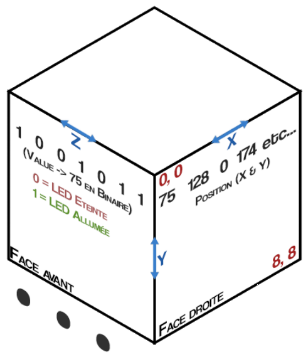
\includegraphics[width=8cm]{./img/schemaCube.png}
	\caption{Représentation 3D du tableau \emph{CubeLED}}
	\label{3dArray}
\end{figure}
\newpage

\subsection{Format ".cube"}
\noindent Le fichier cube est construit en trois catégories principales :
\begin{itemize}
	\item[*] En-tête du fichier (ASCII)
	\item[*] Images du CubeLED
	\item[*] Luminosité
\end{itemize}
Chaque partie du fichier est séparée par des séparateurs de début et fin. Pour indiquer le début d’une partie, on utilise "\#", pour marquer la fin d’une partie on utilise "\$" par convention.

\vspace{0.5cm}



\begin{flushleft}
	\noindent Voici un schéma représentant la structure du fichier ".cube" :
	\begin{figure}[htp]
		\centering
		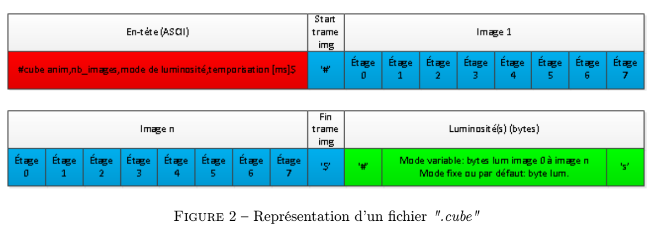
\includegraphics[width=15cm, trim={0 1cm 0 0}, clip]{./img/structureCube.png}
		\caption{Représentation d'un fichier du "\emph{.cube}"}
		\label{structCube}
	\end{figure}
\end{flushleft}

\begin{center}
	\begin{tabular}{|r  l|}
		\hline
		 & \\
		\textbf{\emph{En-tête :}} & Contient les informations relatives à l'animation \\
		\textbf{\emph{Images :}} & Contient les informations sur la position des Leds allumées (par étages) \\
		\textbf{\emph{Luminosité :}} & Si le mode est variable, on indique la luminosité pour chaque image,\\
		 & sinon on indique la luminosité générale du cube. \\
		 & \\
		\hline
	\end{tabular}
\end{center}

\noindent Voici un schéma représentant un étage du cube, un étage contient huit lignes de leds :
\begin{figure}[htp]
	\centering
	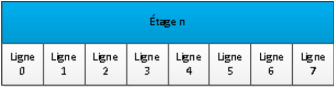
\includegraphics[width=10cm]{./img/structureEtage.png}
	\caption{Représentation d'un étage du \emph{CubeLed}}
	\label{cubeFloor}
\end{figure}

\newpage
% Analyse fonctionnelle
\section{Analyse fonctionnelle}

\subsection{C\#}
Le logiciel sera développé en C\#. Language puissant et utilisé lors de la formation. Il va nous permettre de mettre en place une structure à notre programme en créant des classes et utilisant des bibliothèques. 

\subsection{Esquisse de l'interface}

L'interface (\addRef{interface}) contient les éléments essentiels pour "jouer" avec le cube. Au millieu, dans la partie verte claire, on retrouve le cube à led matérialisé en 3D. L'utilisateur pourra sélectionner les leds du cube et les modifier grâce aux interaction que l'on trouve en dessous.
\vspace{.5cm}

\noindent Dans le groupe boxe, \emph{Options}, on trouve les informations de la led sélectionnée :
\begin{itemize}
	\item \emph{On} : allumer la led
	\item \emph{Off} : étindre la led
	\item \emph{Intensité} : l'intensité de la led
	\item \emph{Changer couleur} : modifier la couleur de la led
\end{itemize}
\vspace{.5cm}

\noindent Dans le second groupe boxe, \emph{Général}, on retrouve les informations par apport à l'application :
\begin{itemize}
	\item \emph{Animation On} : indique qu'une animation sera gérée (plusieurs frame générée)
	\item \emph{Animation Off} : indique que le cube sera une image fixe (une seule frame)
	\item \emph{Play} : met en marche l'animation
	\item \emph{Pause} : suspend l'animation
	\item \emph{Stop} : arrête entièrement l'animation
	\item \emph{Options - Nb image} : nombre d'image pour l'animation
	\item \emph{Options - ms/image} : nombre d'image par milliseconde que le cube doit afficher
\end{itemize}
\begin{figure}[htp]
	\centering
	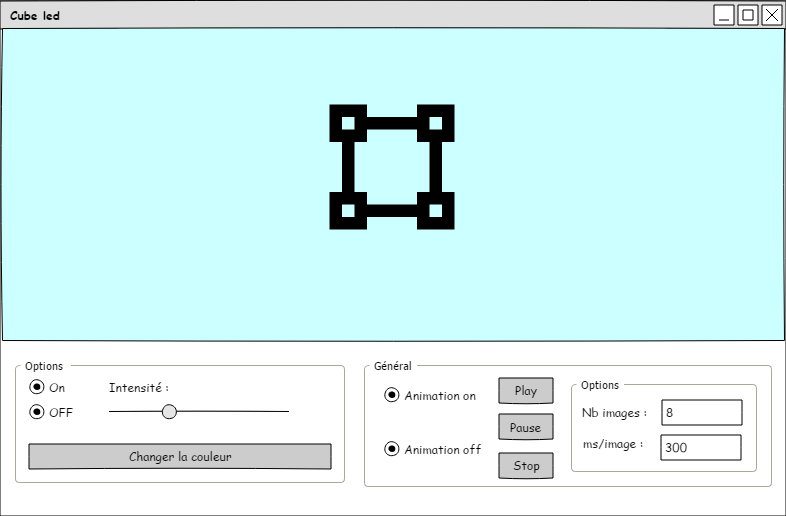
\includegraphics[width=.60\textwidth]{img/windform.png}
	\caption{Esquisse de l'interface du logiciel}
	\label{interface}
\end{figure}

\subsection{\emph{UsbLibraryCfptAdd}}
\emph{UsbLibraryCfptAdd} est une bibliothèque qui permet de communiquer sur une trame USB. Elle a été fournie avec le cube à led pour que l'on puisse communiquer entre le cube à led et le PC. Elle implémente certaine fonctionnalité tels que la détection d'un nouveau périphérique, la communication avec un périphérique donné, la déconnexion d'un périphérique, etc. 

Une bibliothèque créée par nous servira de sur-couche à celle-ci. La bibliothèque pourra alors transformer un format de donnée reçus de notre application, le transformer au format que l'on a besoin. Puis, le format de sortie sera envoyé au cube par la connexion usb.
\newpage

% Analyse organique
\section{Analyse organique}
\subsection{Bibliothèque \clcl}
Pour le processus de communication entre le cube à led et l'application, une bibliothèque C\# a été créée. Cette bibliothèque est une sur-couche de \emph{UsbLibraryCfptAdd}. Elle implémente les fonctionnalités qui permettent la communication spécifique entre le cube et l'application.
\begin{figure}[htp]
	\centering
	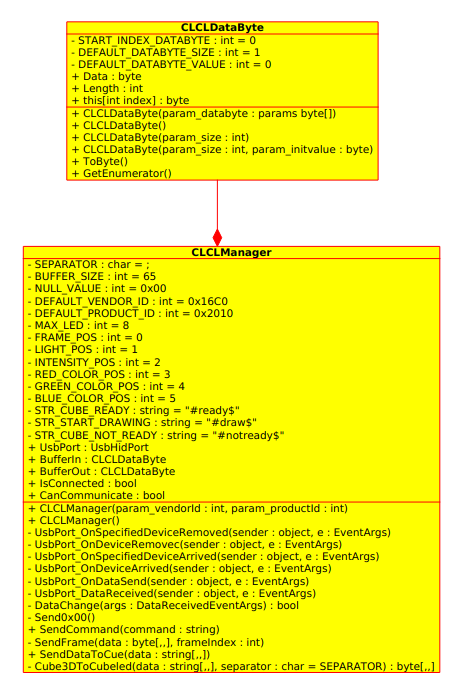
\includegraphics[width=10cm]{./Img/uml_clcl.png}
	\caption{Diagramme \emph{UML} de la bibliothèque \clcl}
	\label{uml_clcl}
\end{figure}

\newpage
\subsection{Monogame}
Monogame est une implémentation \emph{Open Source} du framework Microsoft XNA 4. Le but de monogame dans notre projet est de faciliter la création et la gestion d'objet en 3D. Pour implémenter il suffit de télécharger sur le site "http://www.monogame.net/downloads". Nous avons téléchargé la dernière version disponbile soit la version MonoGame 3.6.

Monogame n'était pas le seul choix possible, au contraire il existe par exemple unity qui permet la création et la gestion simple d'objet 3D (voir même plus simple que monogame), mais nous avons choisis monogame car, implémenter un projet monogame dans un projet windows form avait l'air pour nous beaucoup plus simple avec monogame (voir problèmes rencontrés).

\subsection{Virtualisation du cube en 3D}

\begin{figure}[htp]
	\centering
	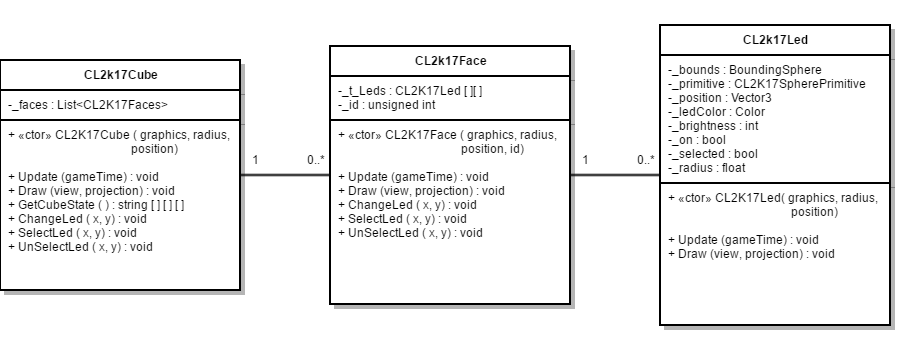
\includegraphics[width=15cm]{./Img/DiagrammeUmlCube.png}
	\caption{Diagramme \emph{UML} du cube 3D}
	\label{uml_clcl}
\end{figure}

\begin{enumerate}
    \item \textbf{Classe CL2K17Led}
    
    Cette classe à deux fonctions enregistrer les données importantes des leds comme par exemple son état (on/off), sa luminosité et encore sa couleur. La deuxième fonction constitue à dessiner ces leds à l'aide d'une librairie télécharger sur "github.com", c'est de la que vient le type SpherePrimitive. 
    
    Le booléan "\emph{selected}" signifie que le focus de l'utilisateur est sur cette led ou non. Elle permet de changer la couleur ou non de la led en question.
    
    La variable de type BoundingSphere est utilisé pour l'intersection en picking, mais cette utilitée n'est pas fonctionnelle (voir problèmes rencontrés). 
    
    \item \textbf{Classe CL2K17Face}
    
    Une face est composée de 64 leds (classe CL2K17Led).
    
    Un "\emph{id} est utilisé pour décaler le dessin de la face des autres faces.
    
    Une face peut changer l'état des leds, malheureusement la luminosité est une option qu'il manque, même si celle-ci est déjà implémentée sur la classe CL2K17led.
    
    \item \textbf{Classe CL2K17Cube}
    
    Un cube contient 8 leds, et permet de renvoyer les données des leds dans un tableau de string 3D sous le format suivant : Frame;State;intensity;Color;
    
    \begin{itemize}
        \item frame : numéro de l'image (exemple : 0)
        \item State : Etat on/off de la led (exemple : true)
        \item intensity : la luminosité de la led en pourcentage (exemple : 55)
        \item Color : couleur de la led en RGB : (exemple : 65535)
    \end{itemize}
    
    Le tableau 3D contient un total de 512 variable string pour les 512 leds du cube.
    
\end{enumerate}

\subsection{Bibliothèque utilisée}

Pour la création de sphère en 3D nous avons opté pour une bibliothèque \emph{Open Source} disponible au lien suivant : https://github.com/CartBlanche/MonoGame-Samples/tree/master/PerformanceMeasuring/Primitives \\

\begin{figure}[htp]
	\centering
	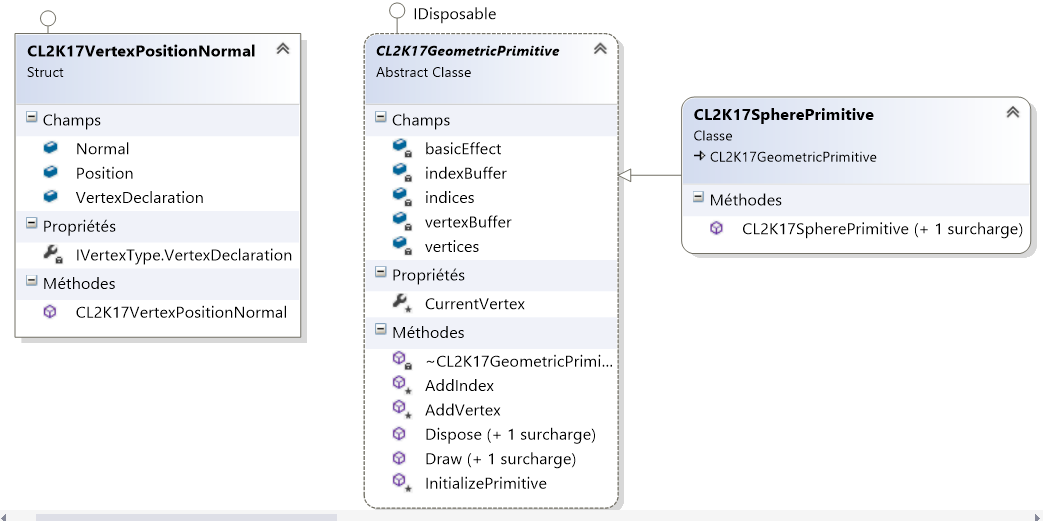
\includegraphics[width=15cm]{./img/diagrammeUmlPrimitive.png}
	\caption{Diagramme \emph{UML} création sphere 3D}
	\label{uml_clcl}
\end{figure}

\begin{enumerate}
    \item \textbf{structure CL2K17VertexPositionNormal}
    
    Pour créer une sphère en 3D, il faut des triangles, pour créer des triangles, il faut des points pour chaque sommet du triangle., c'est la que les vertex prennent tout leur sens. Cette structure aura pourra unique fonction de stocker les points de chaque triangles.
    
    \item \textbf{Classe CL2K17GeometricPrimitive}
    Cette classe permet de dessiner n'importe quel model 3D.
    
    \item \textbf{Classe CL2K17SpherePrimitive}
    Cette classe créer les triangles rejoignant chaque vertex pour créer une sphère.
\end{enumerate}

\newpage

% Conclusion
\section{Conclusion}

\newpage

\section{Source}
\begin{itemize}
	\item Documentation de l'équipe Cube à led de 2015-2016 (existant)
\end{itemize}

% Pictures table
\newpage
\listoffigures


\end{document}
